\documentclass[a4paper,12pt,oneside]{book}

%-------------------------------Start of the Preable------------------------------------------------
\usepackage[english]{babel}
\usepackage{blindtext}

%packagr for hyperlinks
\usepackage{hyperref}
\hypersetup{
    colorlinks=true,
    linkcolor=blue,
    filecolor=magenta,      
    urlcolor=cyan,
}

\urlstyle{same}
%use of package fancy header
\usepackage{fancyhdr}
\usepackage{subcaption}
\setlength\headheight{26pt}
\fancyhf{}
%\rhead{
\includegraphics[width=1cm]{logo}}
\lhead{\rightmark}
\rhead{
\includegraphics[width=1cm]{logo}}
\fancyfoot[RE, RO]{\thepage}
\fancyfoot[CE, CO]{\href{http://www.e-yantra.org}{www.e-yantra.org}}

\pagestyle{fancy}

%use of package for section title formatting
\usepackage{titlesec}
\titleformat{\chapter}
  {\Large\bfseries} % format
  {}                % label
  {0pt}             % sep
  {\huge}           % before-code
 
%use of package tcolorbox for colorful textbox
\usepackage[most]{tcolorbox}
\tcbset{colback=cyan!5!white,colframe=cyan!75!black,halign title = flush center}

\newtcolorbox{mybox}[1]{colback=cyan!5!white,
colframe=cyan!75!black,fonttitle=\bfseries,
title=\textbf{\Large{#1}}}

%use of package marginnote for notes in margin
\usepackage{marginnote}

%use of packgage watermark for pages
%\usepackage{draftwatermark}
%\SetWatermarkText{
\includegraphics{logo}}
\usepackage[scale=2,opacity=0.1,angle=0]{background}
\backgroundsetup{
contents={
\includegraphics{logo}}
}

%use of newcommand for keywords color
\usepackage{xcolor}
\newcommand{\keyword}[1]{\textcolor{red}{\textbf{#1}}}

%package for inserting pictures
\usepackage{graphicx}

%package for highlighting
\usepackage{color,soul}

%new command for table
\newcommand{\head}[1]{\textnormal{\textbf{#1}}}


%----------------------End of the Preamble---------------------------------------


\begin{document}

%---------------------Title Page------------------------------------------------
\begin{titlepage}
\raggedright
{\Large eYSIP2016\\[1cm]}
{\Huge\scshape Automatic Theme Evaluation from videos. \\[.1in]}
\vfill
\begin{flushright}
{\large Keshav Bihani. \\}
{\large Raj Krishna Srivastava. \\}
{\large Khalid Waseem. \\}
{\large Duration of Internship: $ 21/05/2016-10/07/2016 $ \\}
\end{flushright}

{\itshape 2016, e-Yantra Publication}
\end{titlepage}
%-------------------------------------------------------------------------------

\chapter[Project Tag]{Automatic Theme Evaluation from videos.}
\section*{Abstract}
This project aims at automatically evaluating themes that are provided to teams during eYantra competition with help of image and audio processing, without the need for any manual intervention.
Each year, there are many videos submitted before the finals of the competition and automating the evaluation process would help increase number of participants as well as speeding the evaluation process. Moreover this project can find its application in surveillance with slight modifications, and incorporating pattern matching algorithm with audio processing module can help search a small audio clip from a large database within seconds.  

\subsection*{Completion status}
Evaluation of puzzle solver has been achieved. The matlab code generates three log files(.txt files).
\begin{itemize}
  \item The first one is the trace file generated after applying the mean shift algorithm to track the robot and check if it is following the line or not.
  \item Second file contains the the on and off time of the leds as well as the numbers that are picked and deposited.
  \item The third files contains the time of the buzzer beeps that are used to indicate picking up and deposition along with indicating the starting and ending of the run.
\end{itemize} 
These three text files are read as input by a C program which helps to generate the scores.
\section{Software used}
\begin{itemize}
  \item Matlab.
  \item Detail of software: Version R2012a. 
  \item \href{https://www.youtube.com/watch?v=krEPOXPvNIg}{Installation steps}
\end{itemize}

\section{Software and Code}
\href{https://github.com/eYSIP-2016/Automatic-Theme-evaluation-from-videos}{Github link} for the repository of code\\
TranformVideo.m contains the logic for converting the video into orthographic projection.Basic logic is explained below-
Given two images of a coplanar scene taken from two different cameras, how will we determine the planar homography matrix H?How many point correspondences will we require?

    \begin{figure}[h!]
		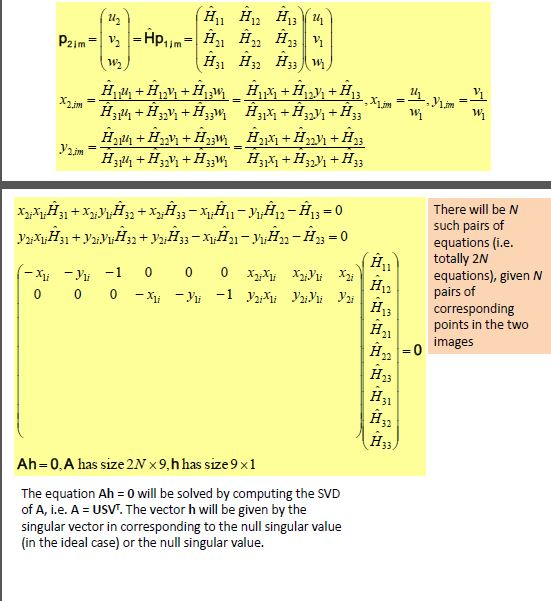
\includegraphics[width=1\linewidth, height=11cm]{Capture-1.JPG}
		\centering
		\caption{Finding Homography Matrix}
	\end{figure}
	
Thereafter once video is converted we will use logic of video tracking specified in the  Mean\_shift\_with\_led\_and\_path.m to generate trace file as well as log file containing on and off time of leds.\\
The project uses the mean shift algorithm to track objects.
Mean shift is a non-parametric feature-space analysis technique for locating the maxima of a density function, a so-called mode-seeking algorithm.
The mean shift iterations are employed to find the target candidate that is the most similar to a given target model, with the similarity being expressed by a metric based on the Bhattacharyya coefficient.
In this algorithm initially a region of interest is selected, then in consecutive iterations it looks in the region of interest and shifts the mean in the direction of increasing density until no more shift is possible, i.e, it has reached the peak of the Probability Distribution Function (densest area).It would be better understood from the following figure.
    \begin{figure}[h!]
		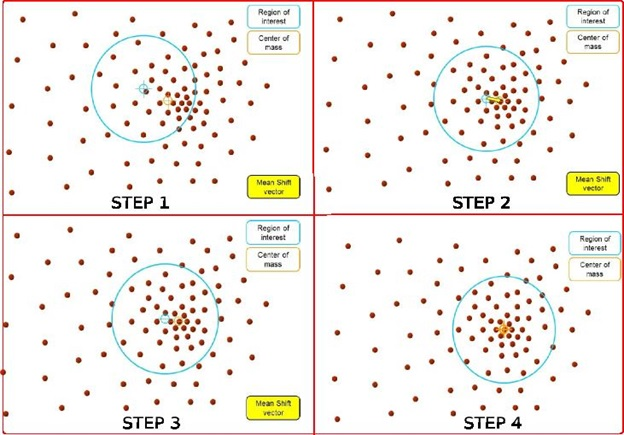
\includegraphics[width=1\linewidth, height=11cm]{ROI.jpg}
		\centering
		\caption{Probability Distribution Function.}
	\end{figure}\\
Robot Tracking using Mean Shift
Mean Shift Algorithm extracts the feature of an object to be tracked. Features can be intensity, color, gradient, etc. In the initial frame the object is chosen. Now a feature of that object is extracted, its histogram is obtained and we come up with a PDF based on this feature. In the next frame we obtain the PDF of the same region and compare it with the previous one using the Bhattacharyya Coefficient. The greater is the similarity between two Distributions, greater is the Bhattacharyya Coefficient. In order to find the new target location we try to maximize the Bhattacharyya Coefficient using mean shift.
    \begin{figure}[h!]
		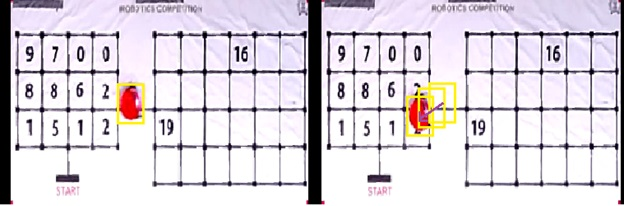
\includegraphics[width=1\linewidth, height=5cm]{ROI1.jpg}
		\centering
		\caption{Robot Tracking using Mean Shift.}
	\end{figure}\\
The audio processing module ampli.m is independent of the above listed processes and generates text files containing on and off time of buzzer.
Firstly the entire signal is converted to frequency domain using fourier transform. 
    \begin{figure}[h!]
		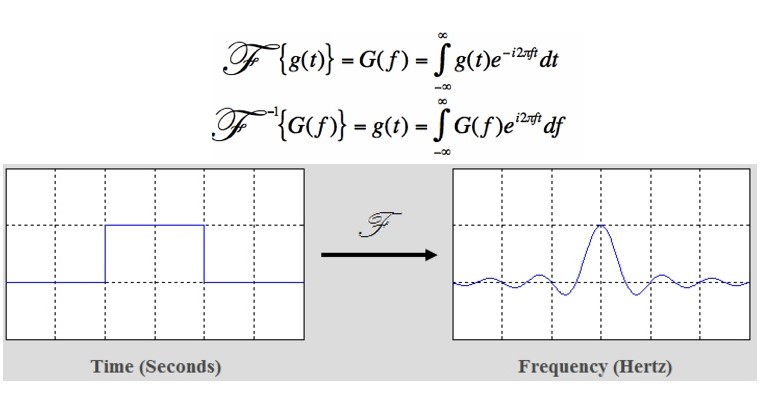
\includegraphics[width=1\linewidth, height=7cm]{Capture-2.jpg}
		\centering
		\caption{Fourier Transform}
	\end{figure}\\
Then we figure out the frequency of buzzer to near about 2.7kHz to 3kHz. Using band pass filter we filter out frequencies in this range and then output the time in a file. Choice of design of the filter and values of different parameters can be found \href{http://in.mathworks.com/help/dsp/ref/bandpassfilter.html}{here}.\\
Using the log files as input,there is C code that generates the score accordingly.
\section{Use and Demo}
\textbf{Final Setup Image.}
    \begin{figure}[h!]
		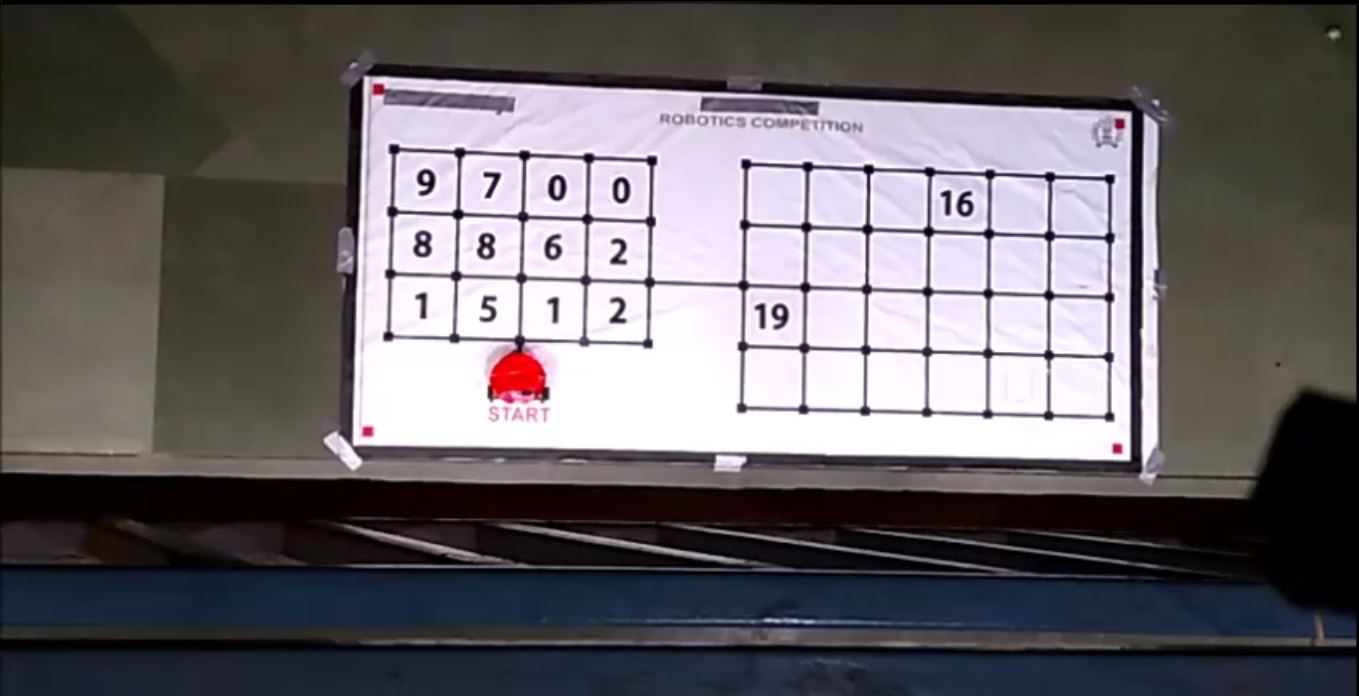
\includegraphics[width=1\linewidth, height=8cm]{Capture.JPG}
		\centering
		\caption{Testing Purpose}
	\end{figure}\\
\textbf{User Instruction for demonstration.}
\begin{itemize}
  \item The position of the arena should be as shown with all the corners visible.
  \item 4cm thick black chart paper must be pasted on the borders of the arena.
  \item Four 2cmx2cm red markers need to be pasted on four corners.
  \item Camera should be entirely stable without any movement and it should be above directly above the arena.
  \item Adequate lightening must be present and there should not be much variation in conditions during filming the video.
  \item The robot should be covered with red colored paper as shown in the image.
\end{itemize}
\textbf{Demonstration Videos.}\\
\href{https://youtu.be/vaqDc_Qd9p8}{Original video with theme implemented.}\\
\href{https://youtu.be/ZgN-Ncc9VRw}{Part of the original video that is being processed.}\\
\href{https://youtu.be/vI5nk7CcUwI}{Homographed Video of task.}\\
\href{https://youtu.be/gpSy3z4Rkdc}{Object tracking implemented on the video.}

\section{Future Work}
\begin{itemize}
\item First of all we need to implement parallel processing in our code since the time for evaluation is humongous to be of any practical use.
Parallel processing is useful when previous outputs do not affect the present inputs.\\
Here we know each frame is represented as matrix and to transform it to orthographic projection we perform operations on each point of the matrix.Now each point is independent to any other point in matrix and operations on them can be done parallely via GPU.
\item Secondly relying just on image processing is not going to allow us achieve our goal of making this evaluation generic. We can incorporate machine learning as well.Machine learning is a type of artificial intelligence (AI) that provides computers with the ability to learn without being explicitly programmed. Machine learning focuses on the development of computer programs that can teach themselves to grow and change when exposed to new data.\\
We can use concepts of ML to identify the arena, the robot and even to identify a perfect run(i.e by giving it samples of prefect task completion).This reduces the risk of errors due to lightening conditions.\\
Support Vector Machines(SVM) are best suited for achieving this task.A SVM is a discriminative classifier formally defined by a separating hyperplane. In other words, given labeled training data (supervised learning), the algorithm outputs an optimal hyperplane which categorizes new examples.More about it can be found on this \href{http://docs.opencv.org/2.4/doc/tutorials/ml/introduction_to_svm/introduction_to_svm.html}{link}
\item Lastly state based evaluation will help us achieve the final goal of making this process generic.
\end{itemize}

\section{Bug report and Challenges}
\begin{itemize}
\item The audio processing module isn't accurate. It would produce correct results every 7 out of 10 times. Rest of the time minor changes in thresholding needs to be done to get desired result.
\item Another problem with the code is that the algorithm used isn't optimized. The pre-processing time is too much to be of any practical use.
\item Change in lightening condition during videos pose an large risk of error generation.
    \begin{figure}[h!]
		\begin{subfigure}{0.4\textwidth}			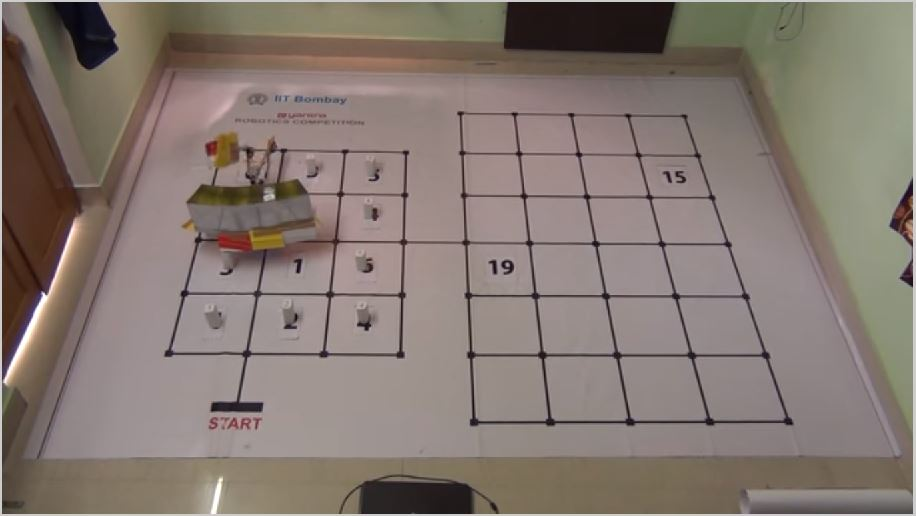
\includegraphics[width=1\linewidth, height=2.5cm]{1.JPG}
			\caption{Earlier}
		\end{subfigure}
		\begin{subfigure}{0.4\textwidth}
			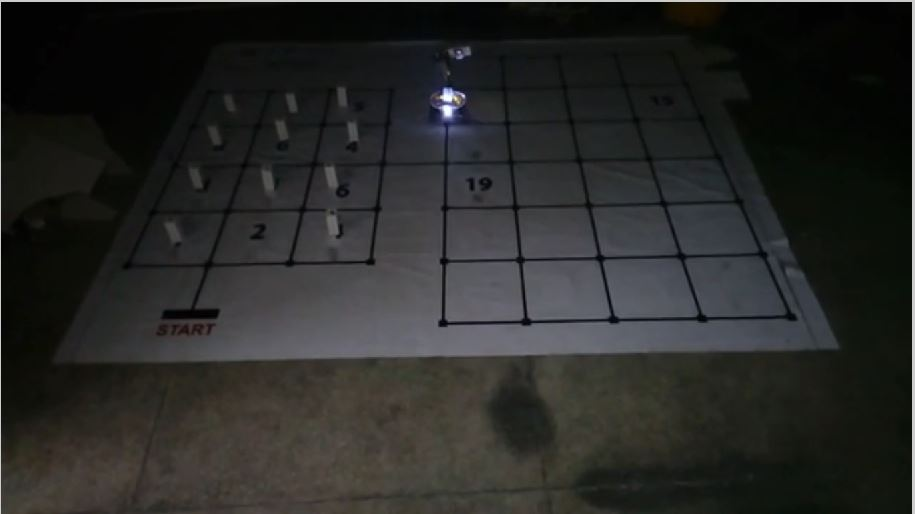
\includegraphics[width=1\linewidth, height=2.5cm]{3.JPG}
			\caption{Later}
		\end{subfigure}
	\end{figure}	
	 \begin{figure}[h!]
		\begin{subfigure}{0.4\textwidth}
			
\includegraphics[width=1\linewidth, height=2.5cm]{11.JPG}
			\caption{Thresholding earlier image}
		\end{subfigure}
		\begin{subfigure}{0.4\textwidth}
			
\includegraphics[width=1\linewidth, height=2.5cm]{33.JPG}
			\caption{Thresholding later with same threshold values}
		\end{subfigure}
	\end{figure}
\end{itemize}

\begin{thebibliography}{li}
\bibitem{wavelan97}
Dr. Niket Kaisare
{\em \href{https://www.youtube.com/watch?v=pj4KKLUMIAg&list=PLa8a_8vztYc7aK6H4bpQTbOqelVIND9Aw}{Introduction to Matlab}}.
\bibitem{wavelan97}
Dorin Comaniciu, Visvanathan Ramesh,
{\em \href{http://comaniciu.net/Papers/MsTracking.pdf}{Research paper on mean shift}}.
\bibitem{wavelan97}
 Rashi Agrawal
{\em \href{https://www.youtube.com/watch?v=-cSVGwAwZZ4&list=PLEo-jHOqGNyUWoCSD3l3V-FjX9PnHvx5n}{Introduction to DIP using Matlab}}.
\bibitem{wavelan97}
 Dr. Mubarak Shah
{\em \href{https://www.youtube.com/watch?v=M8B3RZVqgOo}{UCF Computer Vision Video Lectures}},
2012.
\bibitem{wavelan97}
Mathworks Community
{\em \href{http://in.mathworks.com/help/signal/examples/practical-introduction-to-frequency-domain-analysis.html}{Audio Processing.}}
\bibitem{wavelan97}
Wikipedia
{\em \href{https://en.wikipedia.org/wiki/Support_vector_machine}{Support Vector Machine.}}
\bibitem{wavelan97}
Google
\end{thebibliography}


\end{document}

